\section{Joint Job Loss within Couples}\label{sec:jointloss}

\subsection{The monthly hazard}

Among couples in which both spouses work, a wife loses her job in the same month as her husband in 5.45\% of the
months in which he loses his, against 0.54\% when he keeps his: ten times as often, and 9.4 times what independent
risks would imply. With state $\times$ month fixed effects the excess is 4.0 percentage points (0.040$^{***}$, s.e.\
0.002), and with state $\times$ month $\times$ wife's industry fixed effects, which compare wives in the same industry,
state and month, it is still 3.7 points (0.037$^{***}$): the joint loss is not the local business cycle. It is 3.4
points (0.034$^{***}$) without the pandemic years 2020--21, it is positive in all 51 states (significant in 46), and it is
larger in recessions (6.7 against 3.6 points; difference 0.031$^{***}$).

Figure~\ref{fig:cps_hazard} shows the timing. Relative to the month in which the husband loses his job, the wife's
excess risk of losing hers is 0.6, 0.6 and 0.7 percentage points in the three months before, 4.0 points in the same
month and 0.8, 0.6 and 0.8 points in the three months after (all $p<0.001$). The shock hits both spouses in the same month, on top of a
small shared risk around it.

\begin{figure}[htbp]\centering
\IfFileExists{fig_cps_monthly_hazard.pdf}{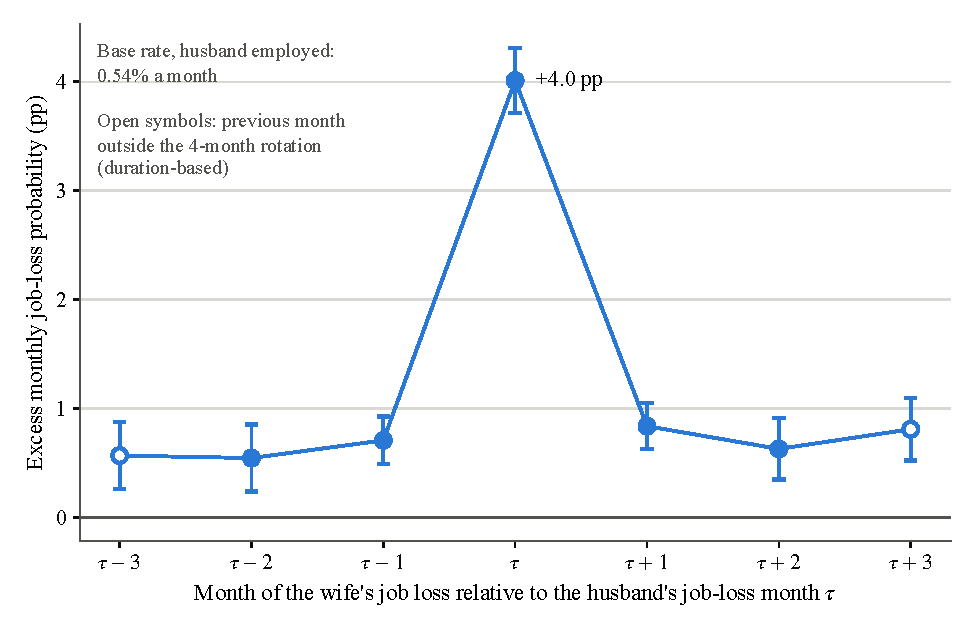
\includegraphics[width=0.85\textwidth]{fig_cps_monthly_hazard.pdf}}%
{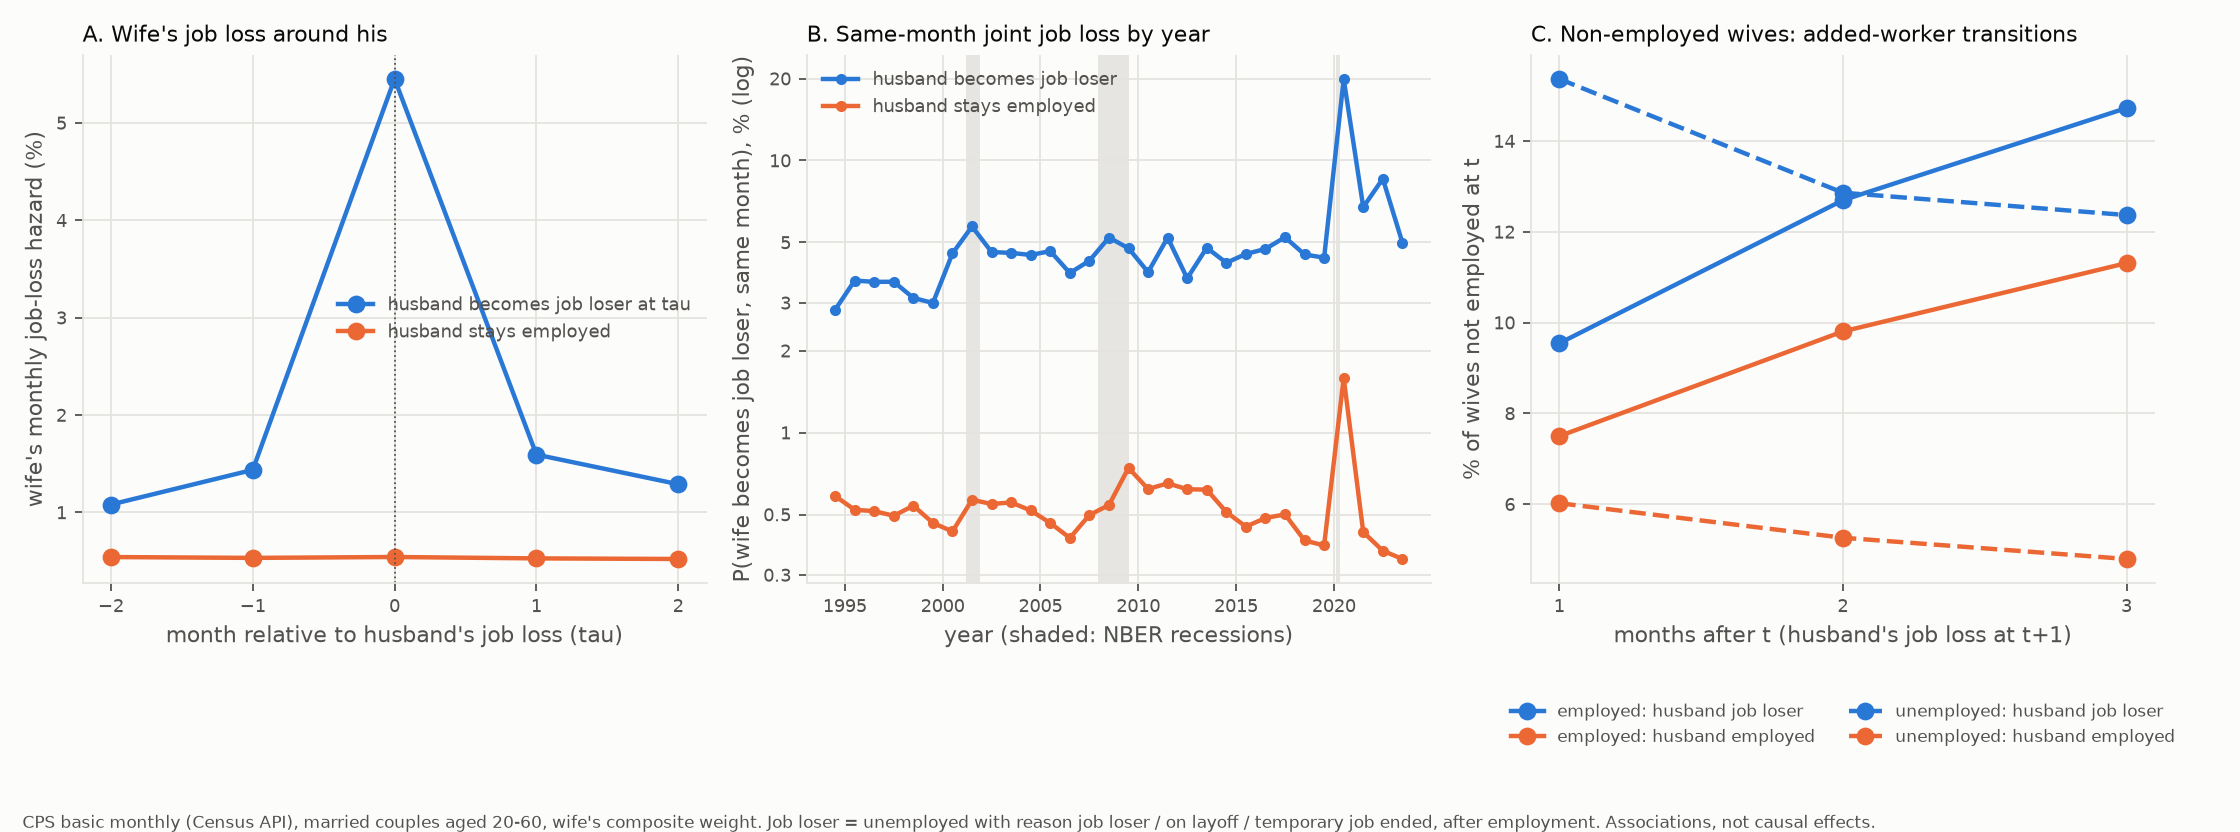
\includegraphics[width=\textwidth]{cps_joint_job_loss.png}}
\caption{The wife's monthly job-loss hazard around her husband's job loss (CPS)}\label{fig:cps_hazard}
\begin{minipage}{0.95\textwidth}\footnotesize Excess probability that the wife loses her job in month $\tau$ relative to
the month in which her husband loses his ($\tau=0$), among couples in which both spouses work; linear probability
models with state $\times$ month fixed effects, 95\% confidence intervals clustered by household. CPS basic monthly
files 1994--2023. At $\tau=\pm3$ the month lies outside the four-month rotation, and a job loss is counted as
unemployment for a job-loss reason lasting four weeks or less (open symbols); the same rule gives 0.041 at $\tau=0$,
against 0.040 from the monthly flows. Code: \texttt{IGE/30.CPSJointJobLoss.py}, \texttt{IGE/37.CPSJointLossChecks.py}.\end{minipage}
\end{figure}

Shared workplaces carry the excess. When the spouses work in the same major industry it rises by 14.8 points
(0.148$^{***}$), and in the same detailed industry 23.0\% of wives lose their job in the month their husband does. The
excess is the same in both races (Black 0.044$^{***}$ on a base of 0.60\%, White 0.038$^{***}$ on 0.54\%; difference
0.006, $p=0.309$), and it does not depend on whether the couple has young children.

\subsection{Reporting, recall layoffs and the season}

Three features of the CPS could produce a joint job loss that is not one: one household member usually reports for
both spouses, a third of the husbands' job losses are temporary layoffs, and some jobs end with the season or the
school year. None of them accounts for the fact (Appendix~\ref{app:robust}, Table~\ref{tab:cps_checks}). The excess is
3.8 points whether the wife or the husband reports the other's job loss. Temporary layoffs account for about a third of
it: without them the excess is 2.7 points, on a base of 0.23\% for permanent job losses. A joint permanent job
loss---both spouses still unemployed two months later, outside temporary layoffs, the summer and the pandemic---is 13
times as likely in the month the husband loses his job as in other months (1.6 points on a base of 0.17\%). Couples who
share a detailed industry, occupation and class of worker, the closest the CPS comes to a common employer, account for
about a third of the excess, so a shared employer plausibly carries a third to a half of it.

\subsection{Displacements with each spouse's own reason}

The PSID measures the same fact with each spouse's own report of why a job ended, over the years around the husband's
displacement (Table~\ref{tab:joint_job_loss}). In the main sample, in which both a window around the event and a
placebo window before it are observed, the husband's displacement raises the probability that his wife is displaced in
the three years around it by 5.2 percentage points (0.052$^{***}$), from a base of 5.8\%, and in the placebo window four
to two years before it by 2.1 points (0.021$^{*}$, $p=0.093$); with couple fixed effects the difference is 3.1 points
(0.031$^{*}$, $p=0.077$). Wives of men who will be displaced four to six years later are already more often displaced in
the placebo window (0.033$^{**}$, $p=0.012$). Part of the excess is therefore a permanent trait of couples who share
risk and part is contemporaneous: stacking both windows, the permanent couple component is 2.0 points (0.020$^{**}$,
$p=0.012$) and the contemporaneous component 3.3 points (0.033$^{**}$, $p=0.036$). In the sample in which only the window around the event is
required the excess is 8.3 points (0.083$^{***}$), and the event study with couple and calendar-year fixed effects puts
the excess in the year of the husband's job loss (3.6 points) and the year after (2.4 points). The CPS, which measures
timing to the month, shows that the contemporaneous part dominates: the leads are 0.6--0.7 points against a
4.0-point spike.\footnote{Couple and calendar-year fixed effects, reference years $-4$ and $-3$; the estimate is already
elevated in year $-2$ (1.8 points, $p=0.07$), consistent with the spouses' reports dating the same events a year apart,
with shocks reaching the workplace first, or with the permanent component. The excess rises across periods, from 0.027
(not significant) in 1984--89 to 0.073$^{***}$ in 1990--99 and 0.095$^{***}$ in 2000--21 (difference 0.069$^{**}$). The rise
is not dating, since more than 97\% of both spouses' reports carry an end year in every period, and not sorting, since
the share of displaced couples in the same sector falls from 0.20 to 0.13; the 1984--89 estimate rests on 175 displaced
husbands. Code: \texttt{IGE/38.PSIDJointLossChecks.py}. Code:
\texttt{IGE/25.JointJobLoss.py}.}

\begin{table}[htbp]\centering\small
\caption{The wife's own job loss around her husband's displacement}\label{tab:joint_job_loss}
\resizebox{\textwidth}{!}{%
\begin{tabular}{lccccccc}
\toprule
 & \begin{tabular}[b]{@{}c@{}}(1) Wife displaced\\$ev-1$ to $ev+1$\end{tabular} & \begin{tabular}[b]{@{}c@{}}(2) Wife displaced\\$ev-4$ to $ev-2$\end{tabular} & \begin{tabular}[b]{@{}c@{}}(3) Wife displaced\\difference\end{tabular} & \begin{tabular}[b]{@{}c@{}}(4) Any job end\\$ev-1$ to $ev+1$\end{tabular} & \begin{tabular}[b]{@{}c@{}}(5) Any job end\\difference\end{tabular} & \begin{tabular}[b]{@{}c@{}}(6) Employer closed\\$ev-1$ to $ev+1$\end{tabular} & \begin{tabular}[b]{@{}c@{}}(7) Employer closed\\difference\end{tabular} \\
\midrule
\multicolumn{8}{l}{\textit{A. All couples}} \\
Husband displaced in $ev$ & $0.052^{***}$ & $0.021^{*}$ & $0.031^{*}$ & $0.122^{***}$ & $0.073^{**}$ & $0.015^{*}$ & $0.008$ \\
 & (0.014) & (0.013) & (0.017) & (0.022) & (0.029) & (0.009) & (0.011) \\
Husband displaced in $ev+4$ to $ev+6$ & $0.007$ & $0.033^{**}$ & $-0.026$ & $0.051^{**}$ & $-0.016$ & $-0.010^{**}$ & $-0.008$ \\
 & (0.012) & (0.013) & (0.016) & (0.022) & (0.023) & (0.005) & (0.007) \\
Husband displaced in $ev$, window-only sample & $0.083^{***}$ &  &  & $0.170^{***}$ &  & $0.019^{**}$ &  \\
 & (0.013) &  &  & (0.018) &  & (0.008) &  \\
Event study, sum of years $-1$ to $+1$ & $0.081^{***}$ &  &  & $0.153^{***}$ &  & $0.021$ &  \\
 & (0.022) &  &  & (0.043) &  & (0.013) &  \\
Control mean & 0.058 & 0.056 & 0.001 & 0.289 & -0.012 & 0.021 & 0.001 \\
Couples & 21,584 & 21,584 & 21,584 & 21,584 & 21,584 & 21,584 & 21,584 \\
\multicolumn{8}{l}{\textit{B. Black couples}} \\
Husband displaced in $ev$ & $0.081^{***}$ & $0.022$ & $0.059^{*}$ & $0.111^{***}$ & $0.090^{*}$ & $0.015$ & $0.010$ \\
 & (0.029) & (0.026) & (0.034) & (0.040) & (0.050) & (0.016) & (0.019) \\
Husband displaced in $ev+4$ to $ev+6$ & $-0.008$ & $0.051^{*}$ & $-0.059$ & $0.033$ & $-0.060$ & $-0.020^{**}$ & $-0.020$ \\
 & (0.025) & (0.029) & (0.039) & (0.045) & (0.047) & (0.009) & (0.017) \\
Husband displaced in $ev$, window-only sample & $0.088^{***}$ &  &  & $0.151^{***}$ &  & $0.017$ &  \\
 & (0.024) &  &  & (0.031) &  & (0.012) &  \\
Event study, sum of years $-1$ to $+1$ & $0.140^{***}$ &  &  & $0.166^{**}$ &  & $0.018$ &  \\
 & (0.036) &  &  & (0.069) &  & (0.021) &  \\
Control mean & 0.078 & 0.080 & -0.001 & 0.291 & -0.013 & 0.027 & 0.000 \\
Couples & 4,920 & 4,920 & 4,920 & 4,920 & 4,920 & 4,920 & 4,920 \\
\multicolumn{8}{l}{\textit{C. White couples}} \\
Husband displaced in $ev$ & $0.036^{**}$ & $0.017$ & $0.019$ & $0.125^{***}$ & $0.065^{*}$ & $0.015$ & $0.008$ \\
 & (0.016) & (0.014) & (0.020) & (0.027) & (0.034) & (0.010) & (0.013) \\
Husband displaced in $ev+4$ to $ev+6$ & $0.010$ & $0.022$ & $-0.012$ & $0.060^{**}$ & $0.003$ & $-0.006$ & $-0.003$ \\
 & (0.013) & (0.014) & (0.017) & (0.025) & (0.026) & (0.006) & (0.006) \\
Husband displaced in $ev$, window-only sample & $0.077^{***}$ &  &  & $0.176^{***}$ &  & $0.020^{**}$ &  \\
 & (0.016) &  &  & (0.023) &  & (0.010) &  \\
Event study, sum of years $-1$ to $+1$ & $0.047^{*}$ &  &  & $0.142^{***}$ &  & $0.023$ &  \\
 & (0.028) &  &  & (0.055) &  & (0.017) &  \\
Control mean & 0.052 & 0.050 & 0.002 & 0.289 & -0.012 & 0.020 & 0.001 \\
Couples & 16,664 & 16,664 & 16,664 & 16,664 & 16,664 & 16,664 & 16,664 \\
\multicolumn{8}{l}{\textit{D. Black $-$ White (pooled, interactions)}} \\
Husband displaced in $ev$ $\times$ Black & $0.042$ & $0.004$ & $0.038$ & $-0.007$ & $0.032$ & $-0.002$ & $-0.001$ \\
 & (0.033) & (0.029) & (0.039) & (0.048) & (0.061) & (0.019) & (0.023) \\
\bottomrule
\end{tabular}}
\begin{minipage}{0.95\textwidth}\footnotesize Unit: a father $\times$ event year $ev$ with his wife employed at baseline; the treated are fathers first displaced (plant closed or moved, laid off or fired) in $ev$, the controls fathers not displaced up to $ev+6$, and the future placebo fathers first displaced in $ev+4$ to $ev+6$. Outcomes: the wife's own report that a job of hers ended because she was laid off or fired or her employer closed (displaced), for any reason (any job end), or because her employer closed, dated in the window of the column; ``difference'' is the window $ev-1$ to $ev+1$ minus the window $ev-4$ to $ev-2$, which removes any permanent difference in the wife's job stability. Event years 1987--2021, both windows observed. OLS with event-year fixed effects. ``Window-only sample'': the same regression among all couples whose window $ev-1$ to $ev+1$ is observed (the placebo window need not be; 26,024 couples, 738 displaced). ``Event study'': sum of the coefficients for years $-1$, $0$ and $+1$ from a regression of the wife's annual job-loss indicator in years $-4$ to $+4$ on displaced $\times$ year dummies with couple and calendar-year fixed effects, reference years $-4$ and $-3$ (event years 1987--2018; figure \texttt{output/joint\_job\_loss\_es.png}). PSID SRC and SEO, unweighted. Standard errors clustered by 1968 family in parentheses. *** $p<0.01$, ** $p<0.05$, * $p<0.1$. Source: \texttt{IGE/25.JointJobLoss.py}.\end{minipage}
\end{table}

\begin{table}[htbp]\centering\small
\caption{Joint job loss: closures, shared labor markets and pre-trends}\label{tab:joint_job_loss_id}
\resizebox{\textwidth}{!}{%
\begin{tabular}{lccccccccc}
\toprule
 & \begin{tabular}[b]{@{}c@{}}(1) Closures\\only\end{tabular} & \begin{tabular}[b]{@{}c@{}}(2) Closures only:\\her employer\\closed\end{tabular} & \begin{tabular}[b]{@{}c@{}}(3) Layoffs\\only\end{tabular} & \begin{tabular}[b]{@{}c@{}}(4) Same\\sector\end{tabular} & \begin{tabular}[b]{@{}c@{}}(5) Same 3-digit\\industry\end{tabular} & \begin{tabular}[b]{@{}c@{}}(6) Same\\occupation\end{tabular} & \begin{tabular}[b]{@{}c@{}}(7) State\\unemployment\end{tabular} & \begin{tabular}[b]{@{}c@{}}(8) Pre-trend\\controls\end{tabular} & \begin{tabular}[b]{@{}c@{}}(9) No self-\\employed\end{tabular} \\
\midrule
\multicolumn{10}{l}{\textit{A. All couples}} \\
Husband displaced & $0.068^{**}$ & $0.054^{**}$ & $0.044^{***}$ & $0.023^{*}$ & $0.030^{**}$ & $0.039^{**}$ & $0.053^{***}$ & $0.048^{***}$ & $0.038^{**}$ \\
 & (0.027) & (0.021) & (0.016) & (0.014) & (0.014) & (0.015) & (0.014) & (0.014) & (0.016) \\
Displaced $\times$ wife in his sector &  &  &  & $0.203^{***}$ &  &  &  &  &  \\
 &  &  &  & (0.055) &  &  &  &  &  \\
Wife in his sector &  &  &  & $-0.016^{***}$ &  &  &  &  &  \\
 &  &  &  & (0.005) &  &  &  &  &  \\
Displaced $\times$ same 3-digit industry &  &  &  &  & $0.282^{***}$ &  &  &  &  \\
 &  &  &  &  & (0.078) &  &  &  &  \\
Same 3-digit industry &  &  &  &  & $-0.032^{***}$ &  &  &  &  \\
 &  &  &  &  & (0.005) &  &  &  &  \\
Displaced $\times$ same occupation group &  &  &  &  &  & $0.083^{**}$ &  &  &  \\
 &  &  &  &  &  & (0.042) &  &  &  \\
Same occupation group &  &  &  &  &  & $-0.015^{***}$ &  &  &  \\
 &  &  &  &  &  & (0.005) &  &  &  \\
Displaced $\times$ $\Delta$ state unemployment (s.d.) &  &  &  &  &  &  & $0.020$ &  &  \\
 &  &  &  &  &  &  & (0.017) &  &  \\
$\Delta$ state unemployment (s.d.) &  &  &  &  &  &  & $0.004$ &  &  \\
 &  &  &  &  &  &  & (0.005) &  &  \\
Wife displaced in $ev-4$ to $ev-2$ &  &  &  &  &  &  &  & $0.086^{***}$ &  \\
 &  &  &  &  &  &  &  & (0.014) &  \\
Control mean & 0.058 & 0.021 & 0.058 & 0.057 & 0.057 & 0.057 & 0.057 & 0.058 & 0.060 \\
Couples & 20,394 & 20,394 & 20,566 & 20,401 & 20,567 & 20,198 & 20,614 & 20,723 & 15,106 \\
\multicolumn{10}{l}{\textit{B. Black couples}} \\
Husband displaced & $0.110^{*}$ & $0.066$ & $0.067^{**}$ & $0.045$ & $0.064^{**}$ & $0.058^{*}$ & $0.081^{***}$ & $0.078^{***}$ & $0.059^{*}$ \\
 & (0.058) & (0.044) & (0.033) & (0.030) & (0.029) & (0.030) & (0.029) & (0.028) & (0.031) \\
Displaced $\times$ wife in his sector &  &  &  & $0.196^{**}$ &  &  &  &  &  \\
 &  &  &  & (0.089) &  &  &  &  &  \\
Displaced $\times$ same 3-digit industry &  &  &  &  & $0.201$ &  &  &  &  \\
 &  &  &  &  & (0.129) &  &  &  &  \\
Displaced $\times$ same occupation group &  &  &  &  &  & $0.147^{*}$ &  &  &  \\
 &  &  &  &  &  & (0.087) &  &  &  \\
Displaced $\times$ $\Delta$ state unemployment (s.d.) &  &  &  &  &  &  & $0.002$ &  &  \\
 &  &  &  &  &  &  & (0.038) &  &  \\
Wife displaced in $ev-4$ to $ev-2$ &  &  &  &  &  &  &  & $0.058^{**}$ &  \\
 &  &  &  &  &  &  &  & (0.024) &  \\
Control mean & 0.078 & 0.027 & 0.078 & 0.077 & 0.078 & 0.077 & 0.079 & 0.078 & 0.082 \\
Couples & 4,557 & 4,557 & 4,627 & 4,576 & 4,605 & 4,489 & 4,655 & 4,671 & 3,907 \\
\multicolumn{10}{l}{\textit{C. White couples}} \\
Husband displaced & $0.051^{*}$ & $0.048^{**}$ & $0.028$ & $0.012$ & $0.011$ & $0.028$ & $0.037^{**}$ & $0.033^{**}$ & $0.023$ \\
 & (0.029) & (0.024) & (0.018) & (0.015) & (0.015) & (0.017) & (0.016) & (0.016) & (0.018) \\
Displaced $\times$ wife in his sector &  &  &  & $0.190^{***}$ &  &  &  &  &  \\
 &  &  &  & (0.070) &  &  &  &  &  \\
Displaced $\times$ same 3-digit industry &  &  &  &  & $0.318^{***}$ &  &  &  &  \\
 &  &  &  &  & (0.097) &  &  &  &  \\
Displaced $\times$ same occupation group &  &  &  &  &  & $0.047$ &  &  &  \\
 &  &  &  &  &  & (0.044) &  &  &  \\
Displaced $\times$ $\Delta$ state unemployment (s.d.) &  &  &  &  &  &  & $0.028$ &  &  \\
 &  &  &  &  &  &  & (0.019) &  &  \\
Wife displaced in $ev-4$ to $ev-2$ &  &  &  &  &  &  &  & $0.093^{***}$ &  \\
 &  &  &  &  &  &  &  & (0.017) &  \\
Control mean & 0.052 & 0.020 & 0.052 & 0.051 & 0.051 & 0.051 & 0.051 & 0.052 & 0.053 \\
Couples & 15,837 & 15,837 & 15,939 & 15,825 & 15,962 & 15,709 & 15,959 & 16,052 & 11,199 \\
\bottomrule
\end{tabular}}
\begin{minipage}{0.95\textwidth}\footnotesize Sample of Table~\ref{tab:joint_job_loss} without the future placebo; outcome: the wife displaced in $ev-1$ to $ev+1$ (column 2: her employer closed). Columns 1--2 keep displaced husbands whose job loss was a plant closure, column 3 those laid off or fired. Columns 4--6 interact the displacement with the spouses working in the same of 16 sectors, the same 3-digit Census industry, or the same of 8 major occupation groups (husband: latest interview in $ev-3$ to $ev$; wife: $ev-6$ to $ev$). Column 7: change in the state unemployment rate in $ev$ (LAUS), in standard deviations among the displaced. Column 8 controls for the husband's hours and labor income at $ev-2$ ($ev-3$ in biennial years) and their change over the two years before, the wife's hours likewise, and her displacement in $ev-4$ to $ev-2$. Column 9 drops couples in which either spouse was self-employed at an interview in $ev-3$ to $ev$. Main effects of the match variables are included in every panel (shown in panel A). OLS with event-year fixed effects; standard errors clustered by 1968 family. *** $p<0.01$, ** $p<0.05$, * $p<0.1$. Source: \texttt{IGE/25.JointJobLoss.py}.\end{minipage}
\end{table}

\begin{table}[htbp]\centering\small
\caption{How often both spouses lose their jobs}\label{tab:joint_job_loss_magnitudes}
\resizebox{\textwidth}{!}{%
\begin{tabular}{lccccc}
\toprule
 & \begin{tabular}[b]{@{}c@{}}(1) P(she is displaced\\$\mid$ he is)\end{tabular} & \begin{tabular}[b]{@{}c@{}}(2) P(she is displaced\\$\mid$ he is not)\end{tabular} & \begin{tabular}[b]{@{}c@{}}(3) Difference\\\end{tabular} & \begin{tabular}[b]{@{}c@{}}(4) Phi\\coefficient\end{tabular} & \begin{tabular}[b]{@{}c@{}}(5) Tetrachoric\\correlation\end{tabular} \\
\midrule
\multicolumn{6}{l}{\textit{A. Same year (interval)}} \\
All couple-years & 0.102 & 0.039 & $0.063^{***}$ & $0.070^{***}$ & $0.237^{***}$ \\
 & & & (0.005) & (0.006) & (0.016) \\
Black & 0.105 & 0.049 & $0.056^{***}$ & $0.064^{***}$ & $0.201^{***}$ \\
 & & & (0.009) & (0.010) & (0.025) \\
White & 0.100 & 0.036 & $0.064^{***}$ & $0.071^{***}$ & $0.248^{***}$ \\
 & & & (0.006) & (0.007) & (0.018) \\
Same sector & 0.211 & 0.028 & $0.183^{***}$ & $0.186^{***}$ & $0.504^{***}$ \\
 & & & (0.022) & (0.020) & (0.032) \\
Different sector & 0.076 & 0.035 & $0.041^{***}$ & $0.047^{***}$ & $0.182^{***}$ \\
 & & & (0.006) & (0.006) & (0.020) \\
Youngest child 0--5 & 0.105 & 0.040 & $0.065^{***}$ & $0.077^{***}$ & $0.245^{***}$ \\
 & & & (0.009) & (0.010) & (0.026) \\
Youngest child 6--17 & 0.091 & 0.041 & $0.050^{***}$ & $0.055^{***}$ & $0.197^{***}$ \\
 & & & (0.009) & (0.010) & (0.028) \\
No child under 18 & 0.108 & 0.037 & $0.072^{***}$ & $0.076^{***}$ & $0.263^{***}$ \\
 & & & (0.009) & (0.010) & (0.025) \\
Annual survey years (to 1996) & 0.090 & 0.039 & $0.051^{***}$ & $0.055^{***}$ & $0.200^{***}$ \\
 & & & (0.007) & (0.008) & (0.023) \\
\multicolumn{6}{l}{\textit{B. Within one year}} \\
All couple-years & 0.181 & 0.091 & $0.090^{***}$ & $0.067^{***}$ & $0.201^{***}$ \\
 & & & (0.008) & (0.006) & (0.015) \\
Black & 0.183 & 0.113 & $0.070^{***}$ & $0.055^{***}$ & $0.151^{***}$ \\
 & & & (0.015) & (0.012) & (0.030) \\
White & 0.180 & 0.084 & $0.096^{***}$ & $0.071^{***}$ & $0.216^{***}$ \\
 & & & (0.009) & (0.006) & (0.016) \\
Same sector & 0.275 & 0.064 & $0.211^{***}$ & $0.151^{***}$ & $0.415^{***}$ \\
 & & & (0.024) & (0.017) & (0.031) \\
Different sector & 0.148 & 0.080 & $0.068^{***}$ & $0.052^{***}$ & $0.168^{***}$ \\
 & & & (0.009) & (0.006) & (0.017) \\
Youngest child 0--5 & 0.206 & 0.097 & $0.109^{***}$ & $0.087^{***}$ & $0.235^{***}$ \\
 & & & (0.015) & (0.012) & (0.026) \\
Youngest child 6--17 & 0.164 & 0.095 & $0.069^{***}$ & $0.051^{***}$ & $0.156^{***}$ \\
 & & & (0.013) & (0.009) & (0.025) \\
No child under 18 & 0.174 & 0.084 & $0.090^{***}$ & $0.065^{***}$ & $0.205^{***}$ \\
 & & & (0.013) & (0.010) & (0.025) \\
Annual survey years (to 1996) & 0.190 & 0.104 & $0.086^{***}$ & $0.059^{***}$ & $0.178^{***}$ \\
 & & & (0.012) & (0.008) & (0.021) \\
\bottomrule
\end{tabular}}
\begin{minipage}{0.95\textwidth}\footnotesize Couple-years: consecutive interviews of the same married couple, both spouses with positive hours in the earlier year, intervals ending 1984--2022 (one year to 1996, two years in the biennial survey; the last row keeps one-year intervals). Panel A: both spouses displaced (closure, layoff or firing) in the same interval; panel B: her displacement within one year either side of the interval. Column 3: OLS of her displacement on his, standard error clustered by 1968 family; columns 4--5: standard errors from 200 bootstrap draws of 1968 families. *** $p<0.01$, ** $p<0.05$, * $p<0.1$. Source: \texttt{IGE/25.JointJobLoss.py}.\end{minipage}
\end{table}


\begin{figure}[htbp]\centering
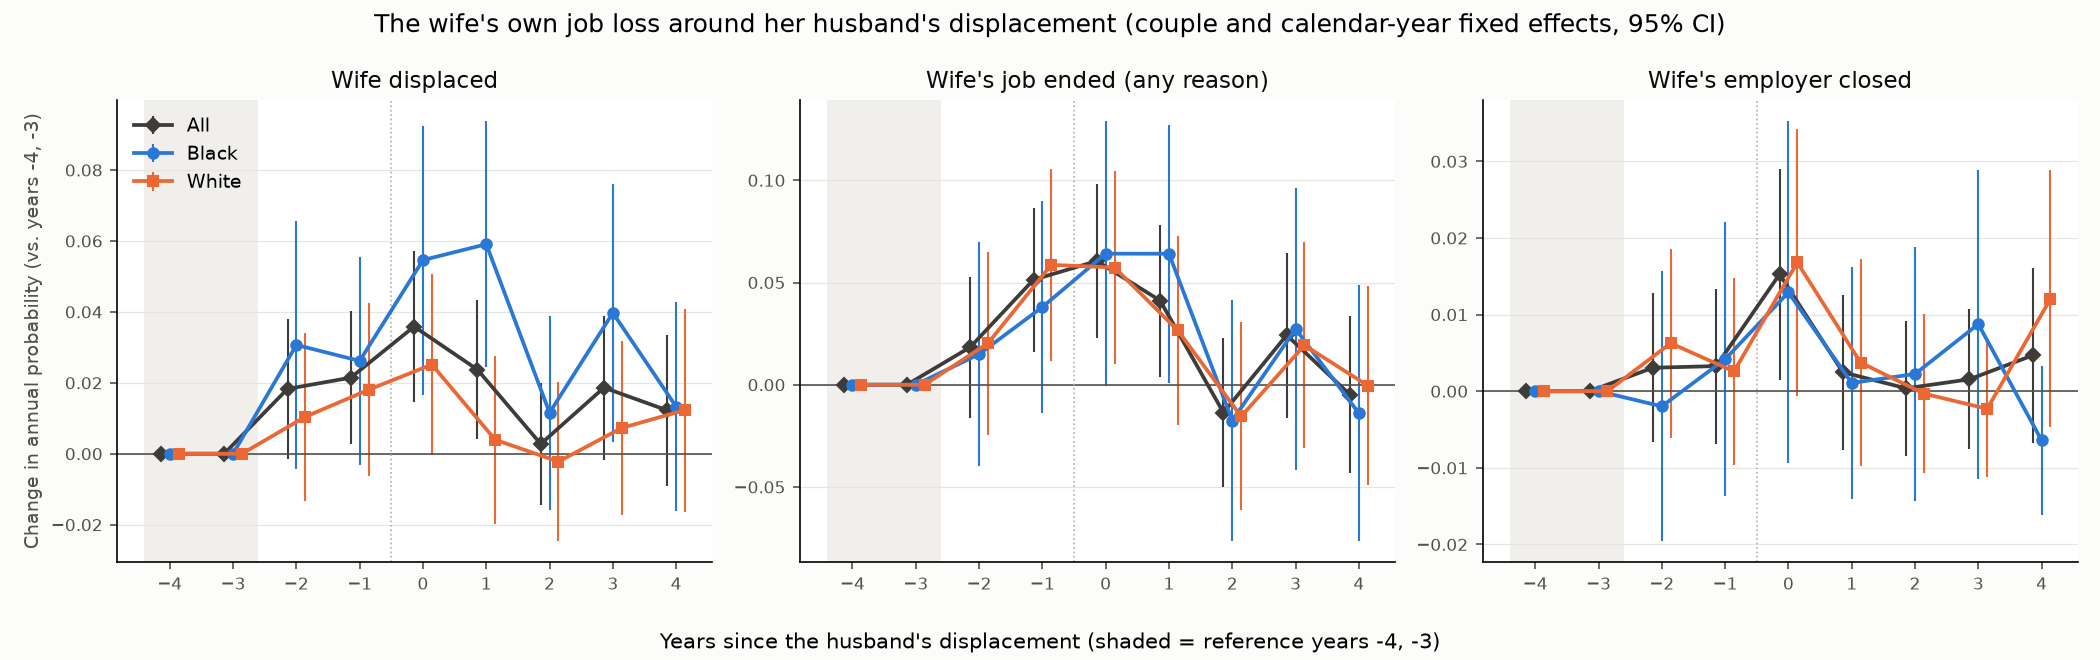
\includegraphics[width=\textwidth]{joint_job_loss_es.png}
\caption{The wife's own job loss around her husband's displacement (PSID)}\label{fig:joint_job_loss}
\begin{minipage}{0.95\textwidth}\footnotesize Event study of the wife's displacement and of her employer's closure,
by year relative to the husband's displacement (reference years $-4$ and $-3$), with 95\% confidence intervals; wives
working at baseline, couple and calendar-year fixed effects. Code: \texttt{IGE/25.JointJobLoss.py}.\end{minipage}
\end{figure}

The channels are the same as in the CPS. When the husband's job loss is a plant closure, the wife's risk of
displacement rises by 6.8 points and the probability that her own employer closes by 5.4 points. Where the spouses work
in the same one of 16 sectors (15\% of couples), the husband's displacement raises her risk by a further 20 points, and
in the same three-digit industry (8\% of couples), the closest the public PSID comes to a common employer, by 28 points.
The change in the state unemployment rate does not moderate it. Controlling for both spouses' hours and earnings before
the job loss leaves an excess of 4.8 points.

\subsection{Two more data sets: the Displaced Worker Supplement and the SIPP}

The CPS Displaced Worker Supplement (1984--2024) records each adult's displacements with the reason and the year in
417,269 couples. A wife was displaced in the same calendar year as her husband in 4.7\% of couples in which he was
displaced and in 1.1\% of the others (an excess of 3.3 points, 0.033$^{***}$), joint plant closings within the same year
are almost ten times as frequent as independent closings would imply, and 68\% of same-year joint closings are in the
same detailed industry. The Survey of Income and Program Participation (SIPP; 2004, 2008 and 2014 panels; 50,692
couples) follows both spouses month by month for up to five years with each job's reason for ending. A wife has an
involuntary separation in the month of her husband's 7.7 times as often as otherwise (an excess of 2.7 points,
0.027$^{***}$), 13 times with a definition close to the CPS one; the excess holds for couples in which both spouses
report for themselves (0.019$^{***}$) and rises by 22 points when the spouses share a detailed industry. In both data
sets the tetrachoric or relative measures match the PSID and the CPS. The excess is the same for Black and White
couples in the CPS and the Displaced Worker Supplement; in the SIPP the same-month excess is smaller for Black couples,
on six joint events, while the twelve-month excess is similar (Appendix~\ref{app:robust}).

\paragraph{By age.} The joint job loss is not a feature of young couples. Outside temporary layoffs, the wife's excess
risk of losing her job in the month her husband loses his is 2.8 percentage points when she is 26--35, 2.4 at 36--45, 2.4
at 46--55 and 2.7 at 56--62 (oldest minus youngest $-0.05$, $p=0.94$); including temporary layoffs it rises with age, from
3.6 to 5.0 points. In the same panel the added worker effect of \citet{bacher2025joint}---the response of a
non-participating spouse to the working spouse's job loss---is 5.6 points (their estimate: 5.55) and declines with age,
from 6.4 points at 26--35 and 7.2 at 36--45 to 1.2 at 56--62, as in their data.\footnote{Couples of a working and a
non-participating spouse, primary earner's transition from employment to unemployment against continued employment,
classification-error adjustment of \citet{bacher2025joint}, 1994--2020; oldest minus youngest $-5.13^{***}$ (s.e.\ 1.03).
Joint job loss: state $\times$ month fixed effects; the same-month joint rate is 6.1 times its value under independence
at 20--25 and 10.7 times at 56--62. Code: \texttt{IGE/50.CPSAddedWorkerByAge.py} (\texttt{output/cps\_awe\_by\_age.md}).}
Older couples, whose non-working spouse barely enters the labor force, remain exposed to the loss of both earners
(Figure~\ref{fig:age_awe_jointloss}).

\begin{figure}[htbp]\centering
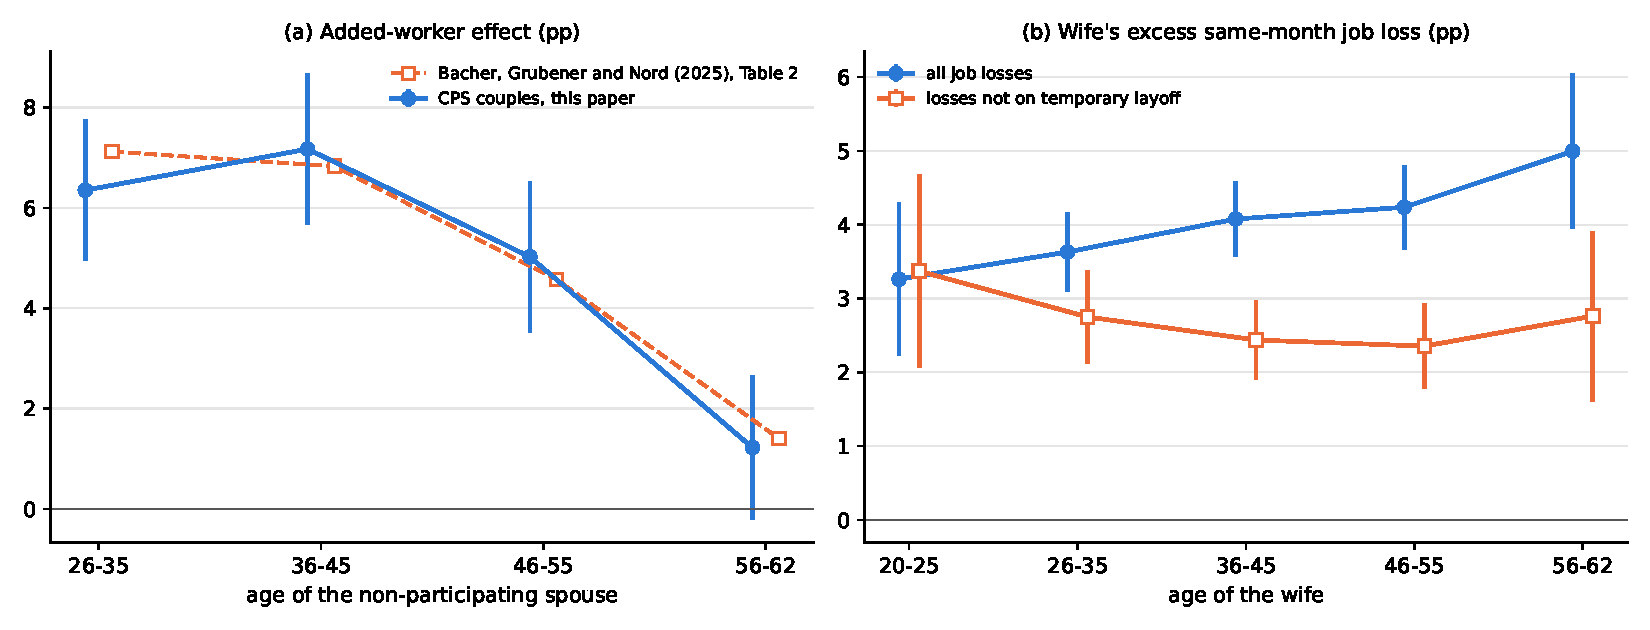
\includegraphics[width=\textwidth]{fig_cps_age_awe_jointloss.pdf}
\caption{The added worker effect and the joint job loss by age (CPS)}\label{fig:age_awe_jointloss}
\begin{minipage}{0.95\textwidth}\footnotesize (a) Added worker effect: the probability that a non-participating spouse
enters the labor force when the working spouse moves from employment to unemployment, minus the same probability when
the working spouse stays employed, by the non-participating spouse's age, with the classification-error adjustment of
\citet{bacher2025joint}, 1994--2020; open squares: their Table~2 (their oldest group is 56--65). Oldest minus youngest
$-5.13^{***}$ (s.e.\ 1.03, $p<0.001$). (b) Excess probability that the working wife loses her job in the month her
husband loses his, by her age; linear probability models with state $\times$ month fixed effects, 1994--2023; open
squares exclude losses on temporary layoff of either spouse. Oldest minus 26--35: all losses 1.45$^{**}$ points (s.e.\
0.63, $p=0.021$; equality across all ages $p=0.11$), losses not on temporary layoff $-0.05$ (s.e.\ 0.68, $p=0.94$;
equality across all ages $p=0.77$). 95\% confidence
intervals clustered by household. Code: \texttt{50.CPSAddedWorkerByAge.py} (\texttt{output/cps\_awe\_by\_age.csv}).
\end{minipage}
\end{figure}

\subsection{Magnitudes for the model}

Table~\ref{tab:joint_job_loss_magnitudes} expresses the result as joint probabilities. Among working couples, the wife
is displaced in 10.2\% of the years in which her husband is and in 3.9\% of the years in which he is not, a tetrachoric
correlation of job loss within the couple of 0.24, which rises to 0.50 when the spouses share a sector. These are the
moments the model targets: a common component of the spouses' displacement risk, larger for couples who share a sector,
on top of a permanent component of couples who share risk.

The joint loss is small in the household's average income loss. A wife's displacement costs her about \$4,600 a year in
labor income; averaged over all displaced families, the joint losses lower wives' earnings by about \$260 a year, about
a fifth of the amount by which family income falls beyond the husband's own earnings and about 2\% of the family's
income loss. It does not explain why wives insure little on average. Its importance lies in the state and the
subgroup in which it occurs: in the month of the shock, when the household's income falls most, and among couples who
share a workplace, where one job loss in five takes both earners. That is where insurance is valued most, and it is
absent from models of family insurance.
